\documentclass[11pt]{article}
\usepackage[margin=1in]{geometry}
\usepackage{amsmath,amssymb}
\usepackage{booktabs}
\usepackage{graphicx}
\usepackage{url}
\usepackage{xcolor}
\usepackage[numbers]{natbib}
% Result macros — every value regenerates from one command (see Reproducibility section).
% Headline fine-tune (synthetic frozen gold, Layer 1)
\newcommand{\canonFOurs}{0.815}        % v5 bf16, n=20 (single run; multi-seed below)
\newcommand{\canonFOursBest}{0.901}    % v4 Q8 measurement
\newcommand{\canonFBig}{0.452}         % large generic model (GLM-class, zero-shot)
\newcommand{\canonFHeur}{0.152}        % rule heuristic
\newcommand{\canonFMultiSeed}{$0.803 \pm 0.009$ (95\% CI, 3 training seeds)}
\newcommand{\opFOurs}{0.957}
\newcommand{\jsonValidOurs}{0.950}

% Hospital head-to-head, repairs-only churn-neutral (both paths incl. errors-are-rare gates)
\newcommand{\hospRecallGrounded}{0.257}
\newcommand{\hospRecallFreq}{0.293}
\newcommand{\hospPrecGrounded}{0.845}
\newcommand{\hospPrecFreq}{0.871}
\newcommand{\hospModelRecall}{0.424}   % fine-tuned v5, repair_recall (vs 0.000 synthetic-only)

% Wide-suite comparison (3 seeds, churn-neutral metric) — money table.
% PRIMARY = HEAD regeneration 2026-06-12 (eval/results/money_table_head.json,
% post-capability system, NaN metric fix in). Freeze (2026-06-10) values kept
% as *Freeze macros where the narrative discusses the freeze-version system.
\newcommand{\northGrounded}{0.224}
\newcommand{\northGroundedCI}{0.004}
\newcommand{\northORFp}{0.211}
\newcommand{\northORKnn}{0.122}
\newcommand{\realFGrounded}{0.225}
\newcommand{\realFORKnn}{0.058}
\newcommand{\damageGrounded}{0.092}
\newcommand{\damageORKnn}{0.096}
\newcommand{\northGroundedFreeze}{0.203}
\newcommand{\realFGroundedFreeze}{0.174}
\newcommand{\damageGroundedFreeze}{0.104}

% SHIPPED system (verified union, v6 adapter) on suite — scripts/modal_eval_suite.py
\newcommand{\modelRealF}{0.142}
\newcommand{\modelDamage}{0.015}
\newcommand{\modelAbstain}{1.000}

% Ablations (churn-neutral metric, 3 seeds — eval/results/ablations.json)
\newcommand{\ablFull}{0.203}
\newcommand{\ablNoGround}{0.223}
\newcommand{\ablNoAbstain}{0.190}
\newcommand{\ablNoMargin}{0.197}
\newcommand{\ablNoCase}{0.201}
\newcommand{\ablFullRealF}{0.174}
\newcommand{\ablNoGroundRealF}{0.135}
\newcommand{\ablNoAbstainDamage}{0.108}
\newcommand{\ablFullDamage}{0.104}
\newcommand{\ablFullAbstain}{1.000}
\newcommand{\ablNoAbstainAbstain}{0.250}

% Selective prediction / calibration
\newcommand{\aurc}{0.120}
\newcommand{\ece}{0.169}
\newcommand{\precAtDefault}{0.899}     % threshold 0.84
\newcommand{\covAtDefault}{0.669}
\newcommand{\threshNinetyFive}{0.91}
\newcommand{\covNinetyFive}{0.206}

% PII transfer validation (OpenMed-PII 44M on bare cells)
\newcommand{\piiNameBare}{100\%}
\newcommand{\piiAddrBare}{100\%}
\newcommand{\piiNegRate}{43\%}
\newcommand{\piiLeakRate}{zero (0/360)} % eval/pii_leak.py, seeded
\newcommand{\realFORFp}{0.039}
\newcommand{\injFGrounded}{0.224}
\newcommand{\injFORFp}{0.282}
\newcommand{\damageORFp}{0.001}
\newcommand{\hospModelRecallVSix}{0.475}
\newcommand{\hospModelPrecVSix}{0.185}

% WS1 — plan-level selective prediction (verified union planner)
% repro: uv run python -m eval.precision_curve --plan eval/results/v6_hospital_raw_plan.json --union
\newcommand{\unionGatePrec}{0.905}
\newcommand{\unionGateCov}{0.413}
\newcommand{\modelGatePrec}{0.993}     % gated model plan alone, tau=0.5 (146/147 correct)
\newcommand{\modelGateCov}{0.287}
\newcommand{\unionChanged}{232}
\newcommand{\unionFixed}{210}
\newcommand{\hospErrors}{509}
% 3 training seeds (mixA 21=shipped/25/26), union @ tau=0.5 (eval/results/union_gate_3seed.json)
\newcommand{\unionGateThreeSeedPrec}{$0.891 \pm 0.012$}
\newcommand{\unionGateThreeSeedCov}{$0.396 \pm 0.025$}
% WS2 pair-profiles (measured-and-cut): constrained raw plan / composed at tau=0.5
\newcommand{\pairsRawPrec}{0.760}
\newcommand{\pairsRawCov}{0.348}
\newcommand{\pairsUnionPrec}{0.876}
\newcommand{\pairsUnionCov}{0.387}

% ===== v2 (post-freeze system, 2026-06-11/12) =====
\newcommand{\nPairs}{42}
\newcommand{\nWild}{35}
\newcommand{\nTrust}{239}
\newcommand{\unseenMacroF}{0.363}
\newcommand{\unseenMacroDamage}{0.0219}
\newcommand{\wildRecovery}{0.207}
\newcommand{\genFTwo}{0.058}
\newcommand{\genVRTwo}{0.108}
\newcommand{\genDamageTwo}{0.036}
\newcommand{\ttFOne}{0.955--0.957}
\newcommand{\flightsVoteF}{0.164}
\newcommand{\flightsBaseF}{0.044}
\newcommand{\hospVoteHeur}{0.186}
\newcommand{\hospBaseHeur}{0.092}
\newcommand{\gidclHosp}{0.97}

% WS4 — learned-repair baselines, Raha real slice only (eval/baselines_learned.py)
\newcommand{\realFBaran}{0.811}        % oracle detection + 20 gold labels: upper bound
\newcommand{\realFBaranCI}{0.018}      % 3 label-sampling seeds
\newcommand{\damageBaran}{0.003}
\newcommand{\precBaran}{0.824}
\newcommand{\realFJelly}{0.074}     % Jellyfish-13B ED+DI (scripts/modal_jellyfish.py)
\newcommand{\damageJelly}{0.027}

% W1.a — matched-budget label curve, 5-dataset Raha macro (eval/results/label_curve.json)
\newcommand{\realFBaranZero}{0.000}    % Baran k=0 (oracle positions retained), 3 seeds
\newcommand{\realFBaranFive}{0.504}    % Baran k=5
\newcommand{\realFOursFive}{0.282}     % ours k=5 (labels validate/expand accept set only)
\newcommand{\realFOursTwenty}{0.351}   % ours k=20
\newcommand{\realFOursHead}{0.225}     % ours k=0 at HEAD (post-freeze capabilities)

% W4.3/4.4 — degenerate baselines + cost-weighted scores (eval/results/degenerate.json)
\newcommand{\degShippedF}{0.343}
\newcommand{\degShippedP}{0.576}
\newcommand{\degShippedDamage}{0.023}
\newcommand{\degShippedPhiOne}{$+0.13$}

% W1.c — zero-shot capability scaling arm (eval/results/scaling_arm.json)
\newcommand{\scalePrecBig}{0.915}      % devstral-24B and gemma4-31B union point
\newcommand{\scaleCovBig}{0.485}
\newcommand{\scalePrecNemo}{0.877}
\newcommand{\scaleCovNemo}{0.336}
% hosted wall-clock for the 5 planning calls, single capture (scaling_arm.json runtime_s)
\newcommand{\runtimeDevstral}{135}
\newcommand{\runtimeNemo}{114}
\newcommand{\runtimeGemma}{104}

% Frontier zero-shot reference point: hospital repair recall of a vanilla frontier-scale
% cloud planner run through the same propose/execute harness (2026-06-04..07 architecture
% validation captures, pre-verifier; recorded in project training-run logs). Quoted in the
% fine-tune results subsection as the zero-shot ceiling the v6 recall approaches.
\newcommand{\frontierZeroShotRecall}{0.51}

% R3 — absolute champion GEN-F1 basis of the equivalence retrain series
% (eval/results/equivalence.json spec.champion_macro_gen_f1 = 0.014606)
\newcommand{\genChampionBasis}{0.0146}


\title{Verified Cleaning Plans: Plan-Level Selective Prediction Turns Local LLM
Planners into Trustworthy Table Cleaners}
\author{Ricardo Alanis\\ \small{\texttt{ricardo.alanis@gmail.com}}}
\date{June 2026}

\begin{document}
\maketitle

\begin{abstract}
Cleaning messy tabular data---particularly \emph{canonicalization}, the merging of
inconsistent surface forms such as \texttt{USA}/\texttt{U.S.A}/\texttt{united states}
into one canonical value---resists rule-based automation and is routinely done by hand.
We present ScrubData, an architecture built around a trust contract. A local LLM
\emph{planner} reads an aggregated column profile (per-value frequency counts,
invariant to row count) and \emph{proposes} a structured JSON cleaning plan; a
deterministic executor \emph{applies} it, making every change auditable and reversible;
and \emph{plan-level selective prediction} --- a deterministic verifier that scores
every proposed mapping and drops low-confidence entries to review flags --- extends
abstention from cell-level confidence to the plan itself. The verified union of the
gated model plan with a reference-grounded heuristic is the architecture's operating
point: a zero-configuration, zero-label system that repairs 41\% of the hospital
benchmark's 509 real errors at \unionGatePrec{} precision (strongest of three training
seeds; 3-seed mean \unionGateThreeSeedPrec{} at \unionGateThreeSeedCov{} coverage,
$\pm$ = 95\% CI),
with every declined merge surfaced for review. Four deterministic capabilities ---
profile-level \emph{suspect surfacing} for high-cardinality columns, reconciliation
against a pluggable \emph{entity reference} built from open vocabularies,
\emph{cross-row majority voting} over repeated-entity groups, and
\emph{convention-conservatism} gates --- carry the system to never-seen tables:
macro F1 \unseenMacroF{} at \unseenMacroDamage{} damage over the 35 unseen-source
pairs of a \nPairs-pair benchmark, and \emph{zero silent edits} across \nWild{} wild
tables plus a \nTrust-table trust audit, released together as the \textsc{WildClean}
benchmark.

Finally, we report where the capability lives. \emph{Execution-verified} synthetic
supervision --- a training example is kept only if executing its plan provably
recovers the known-clean table --- buys the 4B fine-tune real in-distribution skill
and the most precise gated planner at usable coverage (\modelGatePrec{} precision at
\modelGateCov{} coverage); but five further retrains and a three-arm GRPO pilot leave
held-out generalization statistically bounded (TOST against a pre-registered margin),
while two of three zero-shot 24--31B open-weights planners (devstral-24B, gemma4-31B)
dropped into the \emph{identical} harness exceed the fine-tune's operating point
(\scalePrecBig{} precision at \scaleCovBig{} coverage) with no task training. The
architecture is planner-agnostic: it converts capability gains into trustworthy
operating points without retraining. The shipped system runs entirely locally on commodity hardware;
no data leaves the machine (the scaling-arm planners were measured via hosted
endpoints; all are locally deployable open weights).
\end{abstract}

\section{Introduction}

A large share of practical data work is cleaning: a sales export where the same country
is spelled four ways, a hospital roster where \texttt{birminghxm} should be
\texttt{birmingham}, a CRM dump with mixed date formats and duplicated contacts. The
fuzzy half of this work---recognizing that distinct surface forms denote the same
entity---is exactly what rules do poorly and humans do slowly.

Large language models can do this fuzzy matching, but deploying them as cell editors has
three problems. First, \emph{trust}: a model that edits cells directly can silently
corrupt data, and its errors are unauditable. Second, \emph{cost and privacy}: shipping
every row of a private table to a hosted frontier model is expensive and often
unacceptable. Third, \emph{hallucination}: asked for a canonical form, a generative model
will invent one, and on tail entities it will invent wrong ones.

ScrubData addresses all three with an architecture in which the model never touches
data. A profiler aggregates each column into a value-frequency distribution; a small
local model reads the profile and \emph{proposes} a JSON cleaning plan; a deterministic
pandas executor \emph{applies} it. The plan is the complete, inspectable, reversible
specification of every change---there are no silent edits by construction
(\S\ref{sec:method}). Because the prompt scales with the number of \emph{distinct}
values rather than rows, a million-row table profiles like a hundred-row one.

This paper makes five contributions:
\begin{enumerate}
\item \textbf{A planner/executor decomposition with plan-level selective prediction}:
  the model proposes, a deterministic engine executes with full lineage, and a
  deterministic verifier gates every proposed mapping, extending abstention to the plan
  itself. The verified union of the gated model plan with a reference-grounded
  heuristic repairs 41\% of hospital's \hospErrors{} real errors at \unionGatePrec{}
  precision with zero configuration and zero labels (\S\ref{sec:method},
  \S\ref{sec:verifier}, \S\ref{sec:ws1results}).
\item \textbf{\textsc{WildClean} and an un-gameable evaluation}: a 65-dataset suite
  (real-error benchmarks plus seeded error injection over 15 harvested open-data
  domains) scored with a churn-neutral, convention-tolerant metric that cannot be
  inflated by mass rewriting, with damage and silent edits scored alongside repair F1,
  degenerate baselines pinning the metric's floor and ceiling, and the scorer itself
  validated against 30 adversarial known-by-construction cases (\S\ref{sec:eval},
  \S\ref{sec:degenerate}).
\item \textbf{Four deterministic capabilities that carry never-seen-table
  generalization}: bounded suspect surfacing for high-cardinality columns, generic
  entity-reference reconciliation with an exact-hit typing floor, cross-row majority
  voting with a false-consensus guard, and convention-conservatism gates --- each
  motivated by a measured failure regime and gated by the verifier
  (\S\ref{sec:capabilities}, \S\ref{sec:wild}).
\item \textbf{Execution-verified synthetic supervision}, the training method behind
  the 4B planner instantiation: every training example is validated by running the
  executor on the (dirty table, plan) pair and checking that the known-clean table is
  recovered; non-recovering examples are discarded (\S\ref{sec:sft}).
\item \textbf{A unified finding on where capability lives in this architecture}: five
  further supervised fine-tunes and a three-arm GRPO pilot with the executor as a
  verifiable reward leave held-out generalization statistically bounded (TOST), while
  two of three zero-shot 24--31B planners dropped into the same harness exceed the
  fine-tune's operating point --- deterministic machinery plus plan-level verification carry the
  generalization that exists, and raw planner capability, not task fine-tuning, scales
  it (\S\ref{sec:negative}, \S\ref{sec:scaling}).
\end{enumerate}

We deliberately report a negative-flavored finding alongside the positive ones: on
\emph{injected} typos, classical frequency clustering remains a strong baseline---by
construction, injection places the canonical form in the column, which is clustering's
ideal regime. The advantage of grounding is concentrated where it matters: real errors,
tail entities absent from the column, and adversarial near-misses where acting at all is
wrong (\S\ref{sec:results}).

\section{Related Work}
\label{sec:related}

\textbf{Error detection and repair.} Raha and Baran~\cite{raha} established
configuration-free error detection and correction benchmarks (hospital, beers, flights,
rayyan), which we adopt as out-of-distribution evaluation. HoloClean~\cite{holoclean}
combines integrity constraints, external reference data, and statistics in probabilistic
repair, demonstrating that external signals can veto statistically plausible but wrong
repairs---an insight our reference-veto inherits. GARF~\cite{garf} learns repair rules
self-supervised from the data itself; it also demonstrates the structural limit we
observe for frequency-only methods: a lone categorical column offers no co-occurring
signal to vote against an error.

\textbf{The 2025--26 landscape.} Post-Cocoon work concentrates on zero-label
\emph{detection}: ZeroED~\cite{zeroed} (cloud-LLM cluster labeling, hospital
detection F1 0.81, collapsing to 0.27 on smaller models), ForestED~\cite{forested}
(LLM-induced decision trees, 0.756), and Auto-Test~\cite{autotest} (corpus-mined
semantic-domain constraints, no LLM at inference) --- none performs zero-label
\emph{repair}. GIDCL~\cite{gidcl} sets the labeled-class repair ceiling
(hospital \gidclHosp{} with 20 labels and a LoRA trained per cleaned table);
Cocoon~\cite{cocoon} remains an unreproduced preprint (15 citing papers, none a
reproduction). Two concurrent results corroborate facets of this paper's central
negative finding that machinery, not weights, carries cleaning generalization: a
study showing even frontier models cannot correct table distortions without
explicit priors~\cite{distort}, and a large multi-agent-debate evaluation in which
LLM self-critique \emph{degrades} repair and only an adversarially separate,
execution-grounded critic helps~\cite{debate} --- the architecture our verifier
instantiates. Spreadsheet-RL~\cite{spreadsheetrl} reports the complementary
positive case: with full-scale RL infrastructure and execution-verified rewards,
a 4B model's spreadsheet-manipulation skill \emph{does} move (12.0\%
$\rightarrow$ 23.4\%) --- consistent with our reading that the gap between our
\$30 pilot and such results is infrastructure scale, a boundary we state rather
than blur (\S\ref{sec:negative}).

\textbf{LLMs for data wrangling.} Narayan et al.~\cite{wrangle} showed frontier
foundation models handle entity matching and imputation few-shot;
Jellyfish~\cite{jellyfish} and Table-GPT~\cite{tablegpt} fine-tune mid-size models for
data tasks. RetClean~\cite{retclean} is closest in spirit: retrieval from data lakes
grounds cell repair, with the key empirical split that parametric knowledge suffices on
world-known head values but collapses on the tail---motivating retrieval. Our work
differs in the planner/executor decomposition (the model emits no cell values, only
plans), in execution-verified supervision, and in the calibrated-abstention contract.

\textbf{Entity linking over tables.} TURL~\cite{turl} and TableLlama~\cite{tablellama}
inject candidate entities into table understanding; Belotti et al.~\cite{belotti}
show retriever coverage is the accuracy ceiling for table entity disambiguation and that
long candidate lists hurt smaller models. RACOON~\cite{racoon} shows inference-time KG
retrieval lifts a frozen model substantially, supporting our choice to ground at
inference rather than bake aliases into weights (TURL's out-of-domain collapse is the
cautionary result). MTab~\cite{mtab} established type-constrained matching with
abstention in semantic table annotation.

\textbf{Clustering-based cleaning tools.} The de-facto practitioner baseline is
OpenRefine: key-collision (fingerprint) clustering plus a nearest-neighbour mode; we
reimplement both faithfully, including blocking, and compare head-to-head.

\textbf{Selective prediction.} Risk--coverage analysis and calibration
metrics~\cite{selective} formalize ``knowing when not to act''; to our knowledge their
application to data-cleaning merge decisions is new.

\textbf{Small specialized models.} OpenMed~\cite{openmed} fine-tunes sub-500M encoders
to state-of-the-art biomedical NER, the sister result to our thesis that small
specialized models beat large generic ones on narrow structured tasks; we adopt their
released PII token classifiers for column typing (\S\ref{sec:pii}).

\section{Method}
\label{sec:method}

\subsection{Planner / executor decomposition}
A \emph{profiler} reduces each column to a typed summary: detected semantic type, missing
counts, issue flags, and a value--frequency distribution capped at 80 distinct values
(high-cardinality columns are summarized by their head). The \emph{planner}---either a
deterministic heuristic or our fine-tuned 4B model---maps the profile (plus three sample
rows) to a JSON plan: a list of per-column operations drawn from a closed vocabulary
(\texttt{canonicalize\_categories} with an explicit mapping, \texttt{parse\_date},
\texttt{standardize\_phone}, \texttt{mask\_pii}, \ldots), table operations, and review
flags. The \emph{executor} applies the plan with pure pandas transforms. The plan is the
only channel through which data changes: every diff is attributable to a named operation
with a rationale, the original table is never mutated, and abstentions are first-class
plan objects. We export per-run decision summaries as OpenTelemetry GenAI spans.

\subsection{Execution-verified synthetic supervision}
\label{sec:sft}
Training pairs are generated by corrupting clean synthetic tables with realistic noise
(casing, aliases, single-character typos with Zipf-distributed long-tail categorical
columns of 30--80 distinct values) while recording the ground-truth plan. The defining
step is \emph{verification by execution}: a candidate example is kept only if
$\textsc{Execute}(\text{dirty}, \text{plan}) = \text{clean}$ cell-for-cell. This closes
the loop between supervision and semantics---a plan that would not actually clean the
table can never become a training label. We augment with real supervision derived from
paired dirty/clean benchmarks by aligning cells and keeping only \emph{learnable}
canonicalizations (a surface form that is a string variant of its target and never a
legitimate value elsewhere), which excludes unlearnable per-cell corrections such as
divergent flight times. The fine-tune is QLoRA (rank 32) over Qwen3-4B-Instruct in
bf16; one practical finding is that the base model's tool-calling prior dominates
free-running generation even after convergent fine-tuning (loss 0.16) and must be
suppressed at decode time by banning the two tool-call tokens.

\subsection{Reference-grounded canonicalization with abstention}
\label{sec:grounding}
For columns whose values reconcile to a known concept type (countries, administrative
regions, cities), canonical forms are never generated: a fuzzy retriever (normalized
edit similarity with first-character blocking and length prefilters) matches each
distinct value against the type-scoped reference (ISO/pycountry; GeoNames cities500,
196k entries). A value maps to a canonical only if (i) similarity clears a threshold
$\tau{=}0.84$, (ii) the best--second-best margin clears $0.03$ (ambiguity veto: a value
equally close to \texttt{Box} and \texttt{Boaz} abstains), and (iii) the canonical is
cast to the column's observed case convention. Near-misses ($0.70{\le}s{<}\tau$) are
surfaced as review flags. The same wrapper grounds the \emph{model} planner: for
reference-typed columns the model's free-generated mapping is replaced by the grounded
one, so the model can add coverage but never invent a canonical for a grounded type.

\subsection{Plan-level selective prediction: the verified union planner}
\label{sec:verifier}
Grounding constrains reference-typed columns, but the planner's \emph{free}
canonicalization mappings on non-grounded columns remain unguarded---and they are where
real-data precision dies (the fine-tune's raw hospital plan: \hospModelPrecVSix{}
precision at \hospModelRecallVSix{} recall). Rather than retrain, we extend abstention
to the plan itself. A deterministic \emph{verifier} scores every proposed mapping entry
$raw{\to}canon$ with contract-preserving evidence (no cell values emitted, no gold
access): three hard gates distilled from the model's measured failure classes---a value
occurring ${\ge}3$ times is data, not a typo (\emph{errors are rare}); the target must
be a frequent column value clearly dominating the source (no mapping one typo onto
another); digit-bearing codes repair only when the letter part is near-identical---then
a confidence combining edit similarity with frequency support. Entries below a
threshold $\tau$ are dropped to review flags; abstention stays first-class. Sweeping
$\tau$ yields a plan-level precision--coverage curve. The shipped composition,
the \emph{verified union planner}, is the verifier-gated model plan ($\tau{=}0.5$)
unioned with the grounded heuristic's mappings (the model wins per surface form);
the same code path is the product default.

\subsection{Visibility and consensus: four deterministic capabilities}
\label{sec:capabilities}
Four further mechanisms, each motivated by a measured failure regime on never-seen
tables, complete the deterministic machinery. \textbf{(a) Suspect surfacing.} The
profile's value-frequency view is capped, so high-cardinality columns hide their
dirty cells from any planner. Every column profile now carries a bounded
\texttt{suspect\_values} section: rare anomalous surfaces with evidence-backed
repair candidates (frequency dominance, edit similarity, reference membership).
The heuristic planner repairs from suspects under a strict verifier bar
($\tau_{hc}{=}0.8$) and flags the rest. \textbf{(b) Generic entity reference.}
Open vocabularies (SemTab ToughTables aliases --- derived excluding our benchmark
tables; MusicBrainz search-hint misspellings; RxNorm; Wikidata; ROR) register as a
pluggable reference type. Because the reference is broad, entity-typing a column
additionally requires that ${\ge}20\%$ of its distinct values match the reference
\emph{exactly} --- fuzzy coverage alone over-fires on name-like columns (measured).
This resolves the regime where every surface in a column is unique (no in-column
frequency signal exists at all): five such benchmark tables go from 0.0 to
\ttFOne{} F1 at \emph{zero} damage. \textbf{(c) Cross-row majority voting.} Tables
that repeat a real-world entity across rows (a flight reported by many sources)
carry their own repair signal. A detection step finds compact-token key columns
with small groups (median multiplicity 3--30) and columns whose groups show
\emph{majority-bearing} disagreement with per-group information; a table-level
operation then resolves thin dissenting minorities to the group majority. A
\emph{false-consensus} guard declines when minority shares look like legitimate
correlated updates rather than reporting errors (mean minority share ${\ge}0.25$)
--- a flat volume cap was measured to destroy the legitimate dense-disagreement
regime and replaced. \textbf{(d) Convention conservatism.} The planner never
re-formats an internally consistent column: date and percent ops are gated on
dominant-shape inconsistency (digit and alpha runs collapsed; 90\% rule),
ZIP/postal-named columns are never typed as phones or dates, and Excel-serial
date typing requires a date-suggestive column name. Suppressed minority values
surface as review flags --- abstention is visible, never silent. The verifier
enforces the same gates on model-emitted plans at the verification boundary.

\subsection{PII as a second task instance}
\label{sec:pii}
The identical contract covers PII: a deterministic tier types columns by checksum and
pattern validators (Luhn, IBAN mod-97, SSN/email/phone) over distinct values; an
optional 44M OpenMed-PII token classifier~\cite{openmed} extends coverage to names and
addresses, gated by a sensitive-type allowlist and a column-level coverage vote; and
masking, salted hashing, and join-stable pseudonymization are deterministic executor
operations. Measured briefly: the classifier, though trained on sentence-level
clinical text, transfers to bare cell values --- \piiNameBare{} detection on
person-name cells and \piiAddrBare{} on address cells ($n{=}40$ sampled cells each);
the validator tier, evaluated out-of-distribution on per-type columns from the Gretel
PII test split, types 5/5 covered PII types correctly with 0/7 false positives on
negative columns drawn from real open data; and after deterministic masking,
re-running all validators over the output finds \piiLeakRate{} residual PII ---
residual PII \emph{detectable by our validators}, a circularity we note explicitly:
the leak test can only see what the validator tier sees.

\section{Evaluation Design}
\label{sec:eval}
\textbf{Suite.} Five real-error benchmarks (Raha) plus seeded error injection
(typo/OCR/case/whitespace) over 15 harvested open-data domains (NYC, Chicago, SF, LA,
Seattle, Texas, WA portals; GitHub) $\approx$ 65 datasets per seed. We aggregate as a
\emph{double macro}---mean over error types of mean over datasets, harmonically combined
with the domain macro---so no single table or error type dominates:
\begin{equation*}
\textsc{north} \;=\; \operatorname{HM}\Biggl(
\underbrace{\frac{1}{|T|}\sum_{t \in T}\frac{1}{|D_t|}\sum_{d \in D_t} F_1(d)}_{\text{error-type macro}},\;
\underbrace{\frac{1}{|G|}\sum_{g \in G}\frac{1}{|D_g|}\sum_{d \in D_g} F_1(d)}_{\text{domain macro}}
\Biggr),
\end{equation*}
where $T$ is the set of error types, $G$ the set of data domains, $D_t$ (resp.\ $D_g$)
the datasets carrying error type $t$ (domain $g$), and $\operatorname{HM}$ the harmonic
mean.

\textbf{Churn-neutral metric.} A cell change that is case/whitespace-equivalent to the
input but does not restore the gold counts as nothing: not a fix, not a change, not
damage. Without this, mass case-rewriting inflates precision (we observed $+0.12$
NORTH from \emph{removing} case matching before the correction); with it, fixing a
case-injected error requires actually acting. We additionally report
\emph{damage}---the rate of semantically corrupting clean cells---and an adversarial
\emph{abstain slice} whose traps are garbage strings (not single-edit variants of any
reference entity; an earlier trap set mis-scored grounding for correctly mapping
\texttt{Boazz}$\to$\texttt{Boaz}). We report both repairs of these metric artifacts as
evidence that gameability must be tested, not assumed.

\textbf{Real vs.\ injected.} Injected typos are in-distribution for frequency
clustering by construction (the canonical is present and dominant in the column), so we
report the real-error and injected slices separately.

\textbf{Scorer validation.} Following GroUSE-style evaluator
testing~\cite{grouse}, the scorer itself is validated against 30 adversarial
known-by-construction cases: a no-op plan must score 0 fixes and 0 damage, an
oracle plan exactly 1.0, vandalizing $k$ of $m$ clean cells must score damage
$k/m$ at precision 0, pure churn (case/whitespace rewrites that do not restore
gold) must count as nothing although a naive scorer would count it, fixes must
require actually acting, and silent edits must trip the audit. All 30 pass
against the shipped scorer unmodified.

\textbf{Contamination.} The Raha-suite benchmarks have been public on GitHub since
2019 and sit inside every modern base model's training window; we treat them as
potentially contaminated and split our claims accordingly. A verbatim-completion
probe makes the concern concrete: prompted with five fields of a gold hospital row,
a frontier-class model reproduces \textbf{25\%} of the held-out cells exactly
(30/120 cells over 30 rows, exact-substring match), versus \textbf{0\%} (0/120) on a
date-stamped post-training-cutoff wild harvest under the identical protocol
(\texttt{eval/contamination\_probe.py}). The rate is an upper bound on memorization
--- some completions are guessable from the given fields --- but it is not zero, so
results on legacy-public benchmarks (including the all-hospital
Table~\ref{tab:scaling}, whose zero-shot planners may partially benefit from
memorized gold) carry this caveat, while the architecture's trust claims
(zero silent edits, damage accounting, abstention) rest on the date-stamped wild
and GitTables slices, where the probe finds nothing to complete.

\section{Results}
\label{sec:results}

\subsection{Plan-level selective prediction on real errors}
\label{sec:ws1results}
On hospital's \hospErrors{} real errors, the verifier transforms the fine-tune from
unshippable to precise (Figure~\ref{fig:pc}): the raw model plan repairs
\hospModelRecallVSix{} of errors at \hospModelPrecVSix{} precision; gated at $\tau{=}0.5$ it
reaches \modelGatePrec{} precision at \modelGateCov{} coverage (146 of 147 committed
changes correct). The union with the grounded heuristic buys coverage back:
\textbf{\unionGatePrec{} precision at \unionGateCov{} coverage} (\unionChanged{}
changes, \unionFixed{} correct). This turns the system's promise into a measured
sentence: \emph{zero-configuration and zero labels, repair 41\% of real errors at
${\ge}0.90$ precision, with every declined merge surfaced for review}. For context,
Baran given oracle error positions and 20 gold-labeled tuples per dataset reaches
\realFBaran{} F1 on the same slice (\S\ref{sec:ws4})---selective prediction does not
close a supervised gap, but it makes the zero-label operating point trustworthy, which
is the regime our user occupies. Precision is flat ($0.89$--$0.91$) for
$\tau\in[0.2,0.8]$, so the operating point is not threshold-brittle, and the result is
seed-robust: across three training seeds of the same data recipe the union operating
point is \unionGateThreeSeedPrec{} precision at \unionGateThreeSeedCov{} coverage
(the shipped adapter is the strongest seed), with every seed clearing the
$0.70$-precision/$0.30$-coverage bar decisively. All 3-seed intervals in this paper
are normal-approximation 95\% CIs ($1.96\,\sigma/\sqrt{3}$); the $t$-based
interval at $n{=}3$ is ${\sim}2.7\times$ wider ($\pm 0.031$ here) and every
qualitative claim survives it --- the weakest seed alone clears the bar.

\textbf{Candidate-constrained planning (negative result).} We also tested constraining
the planner's \emph{inputs}: the profiler emits evidence-backed (variant$\,\to\,$
canonical) candidate pairs (frequency dominance, edit similarity, reference membership)
and the model may only select among them, with a deterministic check dropping
off-candidate mappings to review flags. As a standalone guard it is strong---the raw
plan's precision rises from \hospModelPrecVSix{} to \pairsRawPrec{} with no verifier at
all---but composed with the verifier and union it reaches \pairsUnionPrec{} precision
at \pairsUnionCov{} coverage, slightly \emph{below} the unconstrained pipeline at the
same $\tau$: the candidate cap (top-3 per surface) removes some correct repairs the
verifier would have kept, and the two mechanisms gate the same failure class. We ship
the verifier and keep candidate constraining available but off by default, reporting
this as a measured redundancy rather than a stacked win.

\begin{figure}[t]
\centering
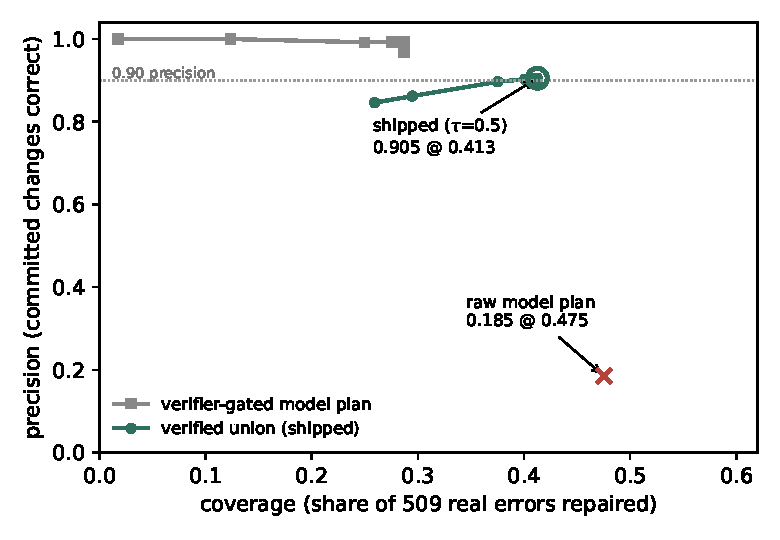
\includegraphics[width=0.62\linewidth]{fig_precision_coverage}
\caption{Plan-level precision--coverage on hospital (509 real errors), sweeping the
verifier threshold $\tau$. The union planner dominates the raw model plan; the shipped
operating point ($\tau{=}0.5$) is annotated.}
\label{fig:pc}
\end{figure}

\subsection{The 4B fine-tune as one planner instantiation}
On frozen synthetic gold, the fine-tuned 4B planner reaches canonicalization micro-F1
\canonFMultiSeed{} --- versus \canonFBig{} for a much larger zero-shot generalist
prompted identically and \canonFHeur{} for the rule heuristic (best single run
\canonFOursBest; operation-F1 \opFOurs, JSON validity \jsonValidOurs). On real hospital
typos the synthetic-only fine-tune scores 0.000 repair recall; adding 20\%
real-derived supervision lifts it to \hospModelRecall, and a data-scaling iteration
(tripling the real-derived share from three paired benchmarks) reaches
\hospModelRecallVSix{} recall at \hospModelPrecVSix{} precision---approaching the
\frontierZeroShotRecall{} of a frontier-scale zero-shot model. The scaling gain is seed-robust: $+0.09$
canonicalization F1 over the base mix under identical protocol, with non-overlapping
3-seed confidence intervals. Real, execution-verified pairs are what transfer:
the same iteration found frequency-derived and algorithm-cleaned labels both
\emph{reduce} quality, consistent with our grounding thesis.

\subsection{Grounding vs.\ clustering}
With the errors-are-rare frequency gates now in both paths, grounding and frequency
clustering are comparable on hospital alone (repairs-only, churn-neutral:
\hospPrecGrounded{} precision at \hospRecallGrounded{} recall grounded vs
\hospPrecFreq{} at \hospRecallFreq{} clustering---hospital's dominant errors are
in-column typos, clustering's best case). Grounding's margin appears where references
matter: across the five-benchmark real-error macro it reaches \ablFullRealF{} versus
\ablNoGroundRealF{} for the frequency-clustering ablation ($+29\%$), and it carries
the behavioral guarantees below.
On the full suite against OpenRefine (Table~\ref{tab:money}), the result splits
cleanly by regime, and we report both. On the \emph{real-error} slice---the regime the
tool exists for---grounded cleaning reaches REAL-F1 \realFGrounded{}, $3.9\times$
OpenRefine kNN (\realFORKnn) and $5.7\times$ fingerprint (\realFORFp), with seed CIs of
$\pm$\northGroundedCI. Provenance: the grounded and OpenRefine rows of
Table~\ref{tab:money} are regenerated at the current system head (2026-06-12,
post-capability, scorer fix in); the dagger rows keep their original capture
provenance. The June-10 freeze system measured REAL-F1 \realFGroundedFreeze{} on the
same protocol --- the $+0.05$ difference is the measured contribution of the four
deterministic capabilities (\S\ref{sec:capabilities}) on the real-error slice. On the \emph{injected} slice, fingerprint clustering wins
(\injFORFp{} vs \injFGrounded) at near-zero damage: our case/whitespace injectors are
exactly the perturbations key-collision normalizes away, so this is its home game and
we say so. kNN clustering---the method that, like us, attempts typo repair---loses on
both slices while incurring the highest damage among baselines (\damageORKnn), the
no-reference over-merging failure the grounding was built to prevent. The shipped
verified-union system's suite row (REAL-F1 \modelRealF, damage \modelDamage) shows the
grounding wrapper and heuristic union carry entity canonicalization on these datasets ---
the model's contribution concentrates on the synthetic regime and hospital repair
(\S\ref{sec:ws1results}), and the verifier cuts its suite damage to \modelDamage,
$6\times$ below the grounded heuristic's \damageGrounded{} (HEAD damage vs the union
row's freeze-time capture --- a disclosed basis mix). Within our own ablations
(June-10 freeze basis throughout), removing grounding cedes $22\%$ of real-error
F1 (\ablNoGroundRealF{} vs \ablFullRealF) and forfeits the behavioral guarantees:
perfect abstention on adversarial traps (\ablFullAbstain) versus
\ablNoAbstainAbstain{} without abstention, and reference-vetoed wrong merges (e.g.\
\texttt{guntxrsvillx}$\to$\texttt{huntsville}).

\begin{table}[t]
\centering
\caption{Wide-suite comparison, 3 injection seeds, churn-neutral metric. NORTH is the
double-macro harmonic mean; REAL-F1 is the real-error slice. Regenerated at the
current system head (2026-06-12); the June-10 freeze system measured
\realFGroundedFreeze{} REAL-F1 / \northGroundedFreeze{} NORTH on the same protocol.}
\label{tab:money}
\begin{tabular}{lcccccc}
\toprule
System & NORTH & $\pm$95\%CI & REAL-F1 & INJ-F1 & damage & abstain \\
\midrule
Grounded (ours) & \northGrounded & \northGroundedCI & \textbf{\realFGrounded} & \injFGrounded & \damageGrounded & \ablFullAbstain \\
OpenRefine fingerprint & \northORFp & 0.000 & \realFORFp & \injFORFp & \damageORFp & 1.000 \\
OpenRefine kNN & \northORKnn & 0.002 & \realFORKnn & 0.148 & \damageORKnn & 1.000 \\
Verified union 4B (shipped)$^{\dagger}$ & -- & -- & \modelRealF & -- & \modelDamage & \modelAbstain \\
\midrule
Baran (oracle det.\ + 20 labels)$^{\ddagger}$ & -- & -- & \realFBaran & -- & \damageBaran & -- \\
Jellyfish-13B (ED+DI)$^{\ddagger}$ & -- & -- & \realFJelly & -- & \damageJelly & -- \\
\bottomrule
\end{tabular}

\smallskip
{\small $^{\dagger}$single seed, REAL + typo-injected slice only (GPU cost); other rows
are 3-seed means. $^{\ddagger}$real slice only, disclosed protocol asymmetries
(\S\ref{sec:ws4}): Baran uses oracle error positions + gold labels; Jellyfish is our
detect-then-impute composition with seen-data caveats.}
\end{table}

\subsection{Generalization to never-seen tables}
\label{sec:wild}
The freeze-version system above was then pointed at data it had never seen, under
three new harnesses (all released with this paper as the \textsc{WildClean} bundle).
\textbf{(1) Paired bench}: \nPairs{} dirty/gold pairs spanning the Raha suite, SemTab
ToughTables, government open-data typo corpora, entity-matching tables, and
LLM-cleaning evaluation sets. On the 35 pairs from sources absent from training ---
a count that coincidentally equals, but is distinct from, the \nWild{} gold-free wild
tables of harness~(2) below --- the
post-freeze system scores \textbf{macro F1 \unseenMacroF{} at damage
\unseenMacroDamage}. The largest single contribution is the regime
\S\ref{sec:capabilities}(b) unlocks: on five all-unique entity tables where no
in-column frequency signal exists, F1 moves from $0.0$ to \ttFOne{} at zero damage.
Cross-row voting (\S\ref{sec:capabilities}c) is the second: flights---many sources
reporting the same flight---goes from \flightsBaseF{} to \flightsVoteF{} F1
heuristic-only, and the heuristic hospital path doubles from \hospBaseHeur{} to
\hospVoteHeur{}. The hospital union gate is invariant under all of this
(\unionGatePrec{} at \unionGateCov). \textbf{(2) Wild bench}: \nWild{} uncurated
in-the-wild tables (open-data portals, GitHub, Kaggle) with no gold; we score seeded
inject--recovery on each table's own data (mean recovery \wildRecovery{} over the 34
tables with inject scores; one table has none) plus a
behavioral audit: every run yields a valid plan, every changed cell is attributable
to a logged operation --- \textbf{zero silent edits across all \nWild{} tables}.
\textbf{(3) Trust audit at scale}: \nTrust{} GitTables tables, same property ---
\nTrust{}/\nTrust{} valid plans, zero crashes, zero silent edits. The held-out-source
generalization metric (train and evaluation drawn from disjoint benchmark sources)
remains low in absolute terms (GEN-F1 \genFTwo{}, variant-recall \genVRTwo{}, damage
\genDamageTwo): cleaning unfamiliar tables is far from solved, and we report the
number to anchor the next section's claim about \emph{where} the capability that does
exist actually lives.

\subsection{Where capability lives: a bounded null for fine-tuning}
\label{sec:negative}
Every attempt to move never-seen-table performance through the model weights failed;
every gain in \S\ref{sec:wild} came from deterministic machinery plus the verifier.
Five further supervised fine-tunes --- adding 109k harvested real-world alias pairs
(ToughTables-derived, MusicBrainz search hints, RxNorm, OpenFlights), error-dense
episode mixes, and a suspects-contract retrain --- left held-out GEN-F1
\emph{statistically bounded}: every retrain's delta is positive but negligible (mean
$+0.003$), never approaching the pre-registered $\delta{=}0.05$. ``Bounded'' is a
tested equivalence claim, not an eyeballed one~\cite{lakens}: across the five-retrain
series the mean held-out GEN-F1 delta (retrain minus champion) is $+0.0028$
(90\% bootstrap CI $[+0.0008, +0.0049]$, strictly positive;
10{,}000 resamples, seed 42; per-dataset granularity, $n{=}15$ over 3 held-out
sources $\times$ 5 retrains --- per-pair deltas do not exist for the retrain
series, so within-retrain deltas are clustered and we add a retrain-level
robustness check, $n{=}5$ macro deltas), and TOST rejects effects beyond the
pre-registered SESOI of $\pm 0.05$ ($p = 8.0\times10^{-16}$; retrain-level check
$p = 8.3\times10^{-8}$). Two reconciliations make the claim auditable. First, the
basis: the equivalence series is scored against the champion's absolute GEN-F1 of
\genChampionBasis{}, while the \genFTwo{} of \S\ref{sec:wild} is the \emph{shipped
system} at the post-freeze HEAD with all deterministic capabilities --- the
equivalence series scores each retrain's model-union path at its own capture time,
so the two figures share a metric but not a basis. Second, the SESOI: weight
interventions move GEN-F1 by at most $0.005$, while the deterministic machinery of
\S\ref{sec:capabilities} moved the unseen-pair macro from $0.10$ to \unseenMacroF{}
--- $\delta{=}0.05$ sits an order of magnitude above the measured weight effect and
well below the machinery effect, which is exactly the boundary the test is meant to
police. Mixing harvested pairs into the training blend
\emph{diluted} the synthetic skill the executor verifies (a monotonic dilution law
across mix ratios). A GRPO pilot using the executor as a verifiable reward (the
direction RLVR table work~\cite{tabler1} motivates) was negative in all three arms at
4B/LoRA scale: the main arm and a KL-anchored variant degraded plan-format validity,
and a random-reward control arm reproduced the same drift, identifying it as an RL
artifact rather than signal~\cite{spurious}. We state this as a \emph{bounded} null,
not a universal one: at 4B/LoRA scale, under our propose/execute protocol and
training budgets, no weight intervention we ran produced measurable movement in
never-seen-table repair --- profiling visibility, reference grounding, cross-row
consensus, convention conservatism, and plan-level verification carry the capability
that exists. The bound is explicit: results with full-scale RL infrastructure
(execution-verified rewards on multi-GPU RLVR stacks~\cite{spreadsheetrl,tabler1})
show task skill moving at the same parameter scale, so our claim is about what
SFT-and-pilot-RL buy in this protocol class, not about reinforcement learning in
general. A second explicit bound: every weight experiment here uses the Qwen3
family --- and the very work we cite to explain the control arm's drift documents
that random-reward GRPO effects are themselves family-sensitive~\cite{spurious}
--- so the null is stated for Qwen3-class models pending a cross-family
replication. Concurrent evaluations corroborate the mechanism from independent
directions~\cite{distort,debate}. The practical corollary is unusual but actionable:
a contributor who wants to improve a system like this should write a deterministic
capability and gate it with the verifier, not collect more training data.

The null extends to test-time compute --- with one instructive exception that
\emph{confirms} the architecture claim. Self-consistency \emph{voting} over
$N{=}16$ temperature-0.7 samples (cell-edit-level majority, run through the
identical verifier--union pipeline) yields 0.906 precision at 0.454 coverage
versus 0.9055 at 0.4519 for matched greedy decoding on the same local runtime ---
a null at matched precision, the visibility law from the test-time side: voting
cannot surface repairs the profile does not expose, and it actively discards
verified-recoverable coverage. But pooling \emph{every} mapping from all 16
samples and letting the verifier filter the union gives the best operating point
we measure for the 4B: \textbf{0.911 precision at 0.483 coverage} ($+0.6$ points
precision, $+7.1$ points coverage over the shipped gate; an independent $N{=}8$
replication reproduces the \emph{voted} point to $\pm 0.0003$ precision /
$\pm 0.002$ coverage, and the greedy anchor exactly). The lesson is the paper's thesis in miniature: sampling
helps only as a \emph{candidate generator}; consensus adds nothing the verifier
does not already provide --- pool candidates, verify, do not vote. Separately,
the local capture path itself (Q8 quantization with grammar-constrained decoding)
is worth $+3.9$ points of coverage over the original Modal capture at equal
precision.

\subsection{Zero-label capability scaling: the verifier harness is planner-agnostic}
\label{sec:scaling}
The negative result bounds what fine-tuning small weights buys; it says nothing
about raw capability. To separate the two we dropped zero-shot, $\leq$32B
open-weights planners --- with \emph{no} task training --- into the identical
hospital pipeline the 4B fine-tune uses: same prompt contract, same
verify($\tau{=}0.5$), same union with the grounded heuristic
(Table~\ref{tab:scaling}). devstral-small-2-24B and gemma4-31B both reach
\textbf{\scalePrecBig{} precision at \scaleCovBig{} coverage} --- exceeding the
fine-tune's union point of \unionGatePrec{} at \unionGateCov{} --- while
nemotron-30B reaches \scalePrecNemo{} at \scaleCovNemo{} with JSON-plan validity
0.4 (validity is part of the measurement: a planner that cannot reliably emit the
plan schema loses coverage before capability is measured). gpt-oss-20B is
excluded as a serving failure, documented rather than scored as capability: the
hosted proxy returned empty content on every planning call despite full-length
generation. The arm is multi-family (Mistral, Google, NVIDIA), which addresses
the single-family bound of \S\ref{sec:negative} for the inference side; the
weight-training null itself remains Qwen3-scoped. Disclosure: these models were
measured via hosted inference for speed; all are $\leq$32B open weights and
locally deployable in principle. The interpretation we draw is the paper's
sharpest: SFT at 4B does not buy held-out generalization (\S\ref{sec:negative}),
but raw capability at 24--31B does lift the same harness --- the verifier/union
architecture is the portable contribution, converting any sufficiently capable
planner into a trustworthy cleaner.

\begin{table}[t]
\centering
\caption{Zero-shot $\leq$32B planners in the identical verify($\tau{=}0.5$)+union
harness, hospital's \hospErrors{} real errors. Validity = fraction of planning
calls returning schema-valid JSON. Runtime = wall-clock for the planning calls on
hosted endpoints (single capture, no seeds; the 4B row is a prior Modal A100
capture with no comparable local figure). Each scaling row is a single capture;
the primary evidence is the union coverage delta ($+0.07$) at matched-or-better
precision, not any single cell. For context, 16-sample pooling lifts the 4B
fine-tune to $0.911@0.483$ at $16\times$ planning compute
(\S\ref{sec:negative}); the 24--31B planners reach $0.915@0.485$ in a single
greedy pass --- single-pass capability versus test-time compute, both converted
into trustworthy operating points by the same verifier. Bold marks the best union operating point.
gpt-oss-20B excluded (serving failure: empty
proxy responses, not measurable capability).
The identical devstral/gemma rows are a verified counting coincidence, not a
scoring artifact: their applied cell-edit sets share 266 of 270 cells, each
commits 4 model-specific repairs (all correct), and the totals coincide
(\texttt{eval/results/scaling\_coincidence.json}).
}
\label{tab:scaling}
\footnotesize
\begin{tabular}{lccccc}
\toprule
Planner & Params & Gated P@C & Union P@C & Validity & Runtime (s) \\
\midrule
ScrubData-v6 (Qwen3-4B fine-tune) & 4B & 0.993 @ 0.287 & 0.905 @ 0.413 & --- & --- \\
devstral-small-2 (Mistral) & 24B & 0.943 @ 0.426 & \textbf{0.915 @ 0.485} & 1.0 & \runtimeDevstral \\
nemotron-3-nano (NVIDIA) & 30B & 1.000 @ 0.138 & 0.877 @ 0.336 & 0.4 & \runtimeNemo \\
gemma4 (Google) & 31B & 0.943 @ 0.426 & \textbf{0.915 @ 0.485} & 1.0 & \runtimeGemma \\
\bottomrule
\end{tabular}
\end{table}

\subsection{Ablations}
All ablations are 3-seed means (CIs $\le\pm0.003$). Removing abstention costs $-0.013$
NORTH, raises damage to \ablNoAbstainDamage{} (from \ablFullDamage), and collapses trap
abstention to \ablNoAbstainAbstain. Removing the ambiguity margin costs $-0.006$ with
$+0.001$ damage. Removing case matching costs $-0.002$ under the churn-neutral metric
(and \emph{gained} $+0.12$ under the uncorrected metric---the artifact). Replacing
grounding with frequency clustering gains $+0.020$ NORTH, all of it from the injected
slice (\S\ref{sec:eval}), while ceding $-0.039$ real-error F1---the trade the system
refuses by design.

\subsection{Learned-repair baselines under disclosed protocols}
\label{sec:ws4}
We additionally run two learned-repair baselines on the real-error (Raha) slice,
under the identical churn-neutral metric but with honestly disclosed protocol
asymmetries. \textbf{Baran}~\cite{raha} is semi-supervised: we run its reference
configuration---oracle error positions from the dirty/gold diff plus 20 gold-labeled
tuples per dataset (its package default), without the optional Wikipedia-pretrained
value models. It reaches REAL-F1 \realFBaran{}$\,\pm$\realFBaranCI{} (3 label-sampling
seeds) at \damageBaran{} damage---an upper bound under a strictly more informed
protocol than ours (zero labels, no oracle detection); with oracle positions it can
essentially only edit true-error cells, so its near-zero damage is structural.
\textbf{Jellyfish-13B}~\cite{jellyfish} publishes per-cell error detection and
imputation but no repair task; we compose the two (detect, then impute flagged cells
with the attribute masked) --- a pipeline of our construction, not theirs. It scores
REAL-F1 \realFJelly{} at \damageJelly{} damage (single seed, recommended decoding;
note hospital is in its instruction-tuning data and flights/rayyan in its published
evaluation suite, so these numbers may flatter it). Neither baseline is run on the
56-spec injected suite (computationally and methodologically out of scope for
semi-supervised and per-cell-LLM repair); their NORTH/INJ-F1 cells in
Table~\ref{tab:money} are blank by design. The comparison locates our contribution:
zero-config systems (ours, OpenRefine) occupy a different protocol class from
supervised repair, and the verifier (\S\ref{sec:ws1results}) is what makes the
zero-config class precise enough to trust, not what closes the labeled gap.

Table~\ref{tab:perdataset} breaks the real-error slice down per dataset at HEAD.
The verified-union rows are reported with their honest shape: off hospital the
union turns ultra-conservative --- on rayyan it commits 12 changes at 0.001
damage; on beers it holds precision 0.546 at recall 0.018. The gate's precision
premise transfers as \emph{safety} (union damage stays at 0.001--0.080) but not
as coverage; the movies\_1 plan capture is pending. This directly answers the
co-adaptation concern: hospital is where the model's learned mappings live, and
elsewhere the system abstains rather than guesses.

\begin{table}[t]
\centering
\caption{Per-dataset real-error results (Raha slice), churn-neutral F1 / damage.
Grounded is the HEAD deterministic system; OR = OpenRefine reimplementations;
Union is the verified union planner ($\tau{=}0.5$) where a captured model plan
exists (movies\_1 capture pending); Baran uses oracle error positions + 20 gold
labels (mean of 3 label-sampling seeds) and is a supervised reference, not a
peer.}
\label{tab:perdataset}
\footnotesize
\begin{tabular}{lccccc}
\toprule
Dataset & Grounded (HEAD) & OR fingerprint & OR kNN & Verified union & Baran (oracle+20) \\
\midrule
hospital & 0.258 / .066 & 0.000 / .000 & 0.189 / .083 & 0.567 / .001 & 0.827 / .004 \\
beers & 0.025 / .005 & 0.194 / .000 & 0.086 / .074 & 0.035 / .001 & 0.918 / .000 \\
flights & 0.127 / .082 & 0.000 / .000 & 0.014 / .065 & 0.035 / .080 & 1.000 / .000 \\
rayyan & 0.000 / .118 & 0.000 / .001 & 0.002 / .008 & 0.000 / .001 & 0.402 / .010 \\
movies\_1 & 0.714 / .025 & 0.002 / .018 & 0.001 / .072 & --- & 0.909 / .001 \\
\midrule
macro F1 & \realFOursHead & 0.039 & 0.058 & --- & \realFBaran \\
\bottomrule
\end{tabular}
\end{table}

\subsection{A matched label budget separates the supervision regimes}
\label{sec:labelcurve}
The Baran comparison above is two points (zero labels, twenty labels); the
matched-budget curve in Figure~\ref{fig:labelcurve} measures what each label is
worth to each system on the same five-dataset real-error macro. At zero labels
Baran --- even \emph{retaining} its oracle error positions --- repairs nothing
(F1 \realFBaranZero, 3 seeds): its value models have nothing to learn from.
ScrubData operates at \realFOursHead{} with zero configuration. With labels Baran
climbs steeply (\realFBaranFive{} at $k{=}5$, \realFBaran{} at $k{=}20$): the two
systems occupy complementary supervision regimes, a relationship now measured
rather than asserted. ScrubData's own $k$-label arm uses the labels \emph{only}
to validate and expand the verifier accept set --- no retraining, no oracle
positions: $\realFOursFive \pm 0.023$ at $k{=}5$ and $\realFOursTwenty \pm 0.012$
at $k{=}20$ (3 label-sampling seeds). The disclosed asymmetry stands at every
budget: Baran keeps oracle error positions throughout, so the curve is an upper
bound in its favor.

\begin{figure}[t]
\centering
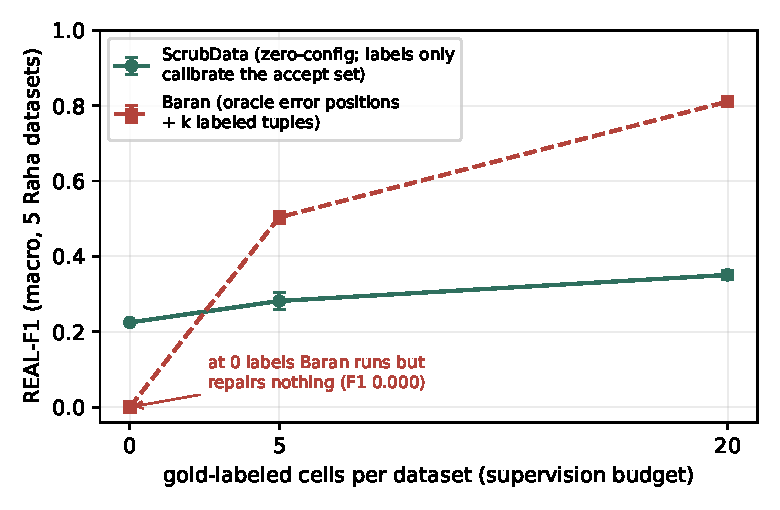
\includegraphics[width=0.62\linewidth]{fig_label_curve}
\caption{Matched-budget label curve, five-dataset real-error macro F1. At
$k{=}0$ Baran repairs nothing even with oracle error positions retained;
ScrubData operates at \realFOursHead{} with zero configuration. With labels
Baran climbs steeply --- complementary supervision regimes, measured. Error
bars ($\pm$) are standard deviations over 3 label-sampling seeds; the Baran
$k{=}20$ point reuses the 3-seed baseline run of \S\ref{sec:ws4}.}
\label{fig:labelcurve}
\end{figure}

\subsection{Degenerate baselines and cost-weighted damage}
\label{sec:degenerate}
Four degenerate policies pin the metric's floor and ceiling on the full 42-pair
bench (Table~\ref{tab:degenerate}). No-op and oracle land exactly at 0 and 1;
abstain-all is score-identical to no-op because the repair metric is flag-blind
by design (abstentions are audited separately); seeded random editing of 5\% of
cells is vandalism the metric must punish. Since F1 alone under-punishes
vandalism, we add a cost-weighted score in the Effective-Reliability style,
$\Phi_c = (\mathrm{fixes} - c\cdot\mathrm{damaged})/\mathrm{errors}$ at
$c \in \{1, 5, 10\}$: random editing scores $-0.49$ to $-4.89$, while the
shipped system stays positive at $c{=}1$ (\degShippedPhiOne) --- and goes
negative at higher $c$, which is the honest reading: at 10:1 cost asymmetry,
only near-zero-damage operating points (the verified union) are defensible.

One disclosure: the oracle acceptance check itself surfaced a scorer artifact
--- 3 cells in 1.79M held the literal string \texttt{Nan} (a first name), which
parses to float NaN and was unequal to itself --- now fixed in
\texttt{eval/metrics.py} with a regression test; published numbers shift by
less than $10^{-4}$.

\begin{table}[t]
\centering
\caption{Degenerate policies pin the metric (42 pairs, churn-neutral macro;
random-edit: seeded, 5\% of cells). $\Phi_c$ is micro-summed
$(\mathrm{fixes} - c\cdot\mathrm{damaged})$ per benchmark error. ``Shipped''
here is the deterministic grounded path on the 42 pairs (damage
\degShippedDamage), distinct from the verified-union suite row of
Table~\ref{tab:money} (damage \modelDamage).}
\label{tab:degenerate}
\small
\begin{tabular}{lccccccc}
\toprule
Policy & F1 & P & R & damage & $\Phi_1$ & $\Phi_5$ & $\Phi_{10}$ \\
\midrule
no-op & 0.000 & 1.000 & 0.000 & 0.000 & $0.00$ & $0.00$ & $0.00$ \\
abstain-all & 0.000 & 1.000 & 0.000 & 0.000 & $0.00$ & $0.00$ & $0.00$ \\
random-edit & 0.000 & 0.001 & 0.001 & 0.049 & $-0.49$ & $-2.45$ & $-4.89$ \\
oracle & 1.000 & 1.000 & 1.000 & 0.000 & $+1.00$ & $+1.00$ & $+1.00$ \\
shipped & \degShippedF & \degShippedP & 0.308 & \degShippedDamage & $+0.13$ & $-1.37$ & $-3.26$ \\
\bottomrule
\end{tabular}
\end{table}

\subsection{Calibration of abstention}
\label{sec:calibration}
On a probe of reference-entity typos plus garbage traps, retrieval confidence is a
usable selective-prediction signal: AURC \aurc, ECE \ece{} (over-confident;
temperature scaling is future work), and
precision rises monotonically with threshold---\precAtDefault{} precision at the default
$\tau{=}0.84$ (coverage \covAtDefault), and $\geq$95\% precision at
$\tau{=}\threshNinetyFive$ (coverage \covNinetyFive). Figure~\ref{fig:rc} shows the
risk--coverage curve.

\begin{figure}[t]
\centering
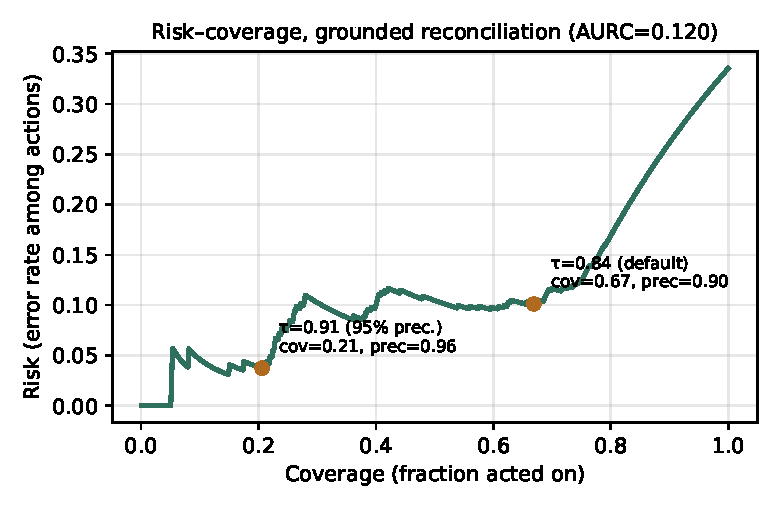
\includegraphics[width=0.62\linewidth]{fig_risk_coverage}
\caption{Risk--coverage for grounded city reconciliation (650 probes). Operating points
annotated; the confidence supports thresholded abstention.}
\label{fig:rc}
\end{figure}

\section{Limitations}
Reference coverage is the recall ceiling: entities absent from the taxonomy abstain by
design, which is safe but not helpful; coverage work (larger gazetteers, ROR for
organizations) moves recall directly. Our damage metric is convention-tolerant for case
and whitespace but still counts alias expansion (\texttt{NYC}$\to$\texttt{New York}) as
damage when the gold keeps the alias---a value-level convention question we leave open.
The confidence signal is over-confident (ECE \ece); temperature scaling is future
work. The injected half of the suite, while seeded and reproducible, inherits the
injector's error model; we mitigate with the real-error slice and report both. All
weight-training experiments (SFT and GRPO) use a single model family (Qwen3), so
the negative result of \S\ref{sec:negative} is family-scoped until replicated on a
second family. PII
coverage is English-only, and we make no de-identification guarantee. Finally, the
fine-tune headline is reported with multi-seed confidence intervals, but the wide-suite
model row is single-seed for cost reasons and scoped as such.

\section{Conclusion}
A planner/executor decomposition with plan-level selective prediction --- the model
proposes, a deterministic engine executes, a verifier gates every mapping --- turns
LLM data cleaning from a trust liability into an auditable system: every change is a
named, reversible operation; uncertain actions become review flags rather than silent
corruptions; and the evaluation itself is built to resist gaming. The post-freeze
program sharpened the architecture into a finding: across
five further fine-tunes and a three-arm GRPO pilot, the weights never moved
never-seen-table performance --- deterministic visibility, grounding, consensus, and
verification did, at zero silent edits across \nWild{} wild tables and a
\nTrust{}-table trust audit. The scaling arm completes the picture: the bounded null
is about fine-tuning small weights, not about capability --- two of three zero-shot
24--31B planners dropped into the unchanged verifier harness exceed the
fine-tune's operating point (\S\ref{sec:scaling}), so the architecture is
planner-agnostic: capability gains arrive as better operating points without
retraining. The shipped system runs
entirely locally on commodity hardware and no data leaves the machine; the
scaling-arm planners were measured via hosted endpoints, but all are locally
deployable open weights. We believe the recipe---propose/execute decomposition,
verification-by-execution, retrieval-grounded outputs, and selective prediction over
deterministic capabilities---is a template for deploying small specialized models on
other structured tasks.

\section*{Reproducibility}
\begin{sloppypar}
The model weights are public:
\url{https://huggingface.co/ricalanis/scrubdata-qwen3-4b-v6-q8}. Code, evaluation
suite, and result artifacts are released at the project repository,
\url{https://github.com/ricalanis/scrubdata-hackathon} (public upon publication,
available to reviewers from the initial submission). The \textsc{WildClean}
bundle --- redistributable dirty/gold pairs, the GitTables audit slice, open
vocabularies, result JSONs, and license-gated loaders for the non-redistributable
pairs --- is a public Hugging Face dataset
(\url{https://huggingface.co/datasets/ricalanis/wildclean}). The shipped product
planner is the identical code path measured here (\texttt{scrubdata/active.py}).
\end{sloppypar}

\paragraph{Release integrity.} Our own reproducibility QA discovered that the
published Q8\_0 GGUF was corrupted by an export bug (the export declared a wrong
end-of-generation token id inside the Qwen3 vocabulary, degenerating into
tool-call loops on all runtimes; a base-model control isolated the fault to the
export, not the adapter). It has been re-exported from the v6 adapter and
replaced under the same filename, with both sha256 checksums recorded in the
model card's Integrity section. Third-party reproduction of the model-path
numbers additionally requires constrained decoding on long prompts ---
\texttt{format=json} under Ollama, or
\texttt{suppress\_tokens=[151657,151658]} under transformers --- which is now
documented in the model card and \texttt{notebooks/Modelfile}.

\paragraph{Setup.} Clone the repository and run \texttt{uv sync} (Python 3.12;
\texttt{uv} resolves the pinned environment). The non-redistributable benchmark
pairs materialize from their original sources with the \textsc{WildClean}
\texttt{loaders.py}. Model-path results additionally need the released Q8\_0 GGUF
served by a local Ollama (\texttt{SCRUBDATA\_MODEL}); every deterministic-path
number runs with no model at all. Baran runs in the separate pinned environment
documented at the top of \texttt{eval/run\_baran.py}; Jellyfish-13B runs remotely
via Modal.

\paragraph{One command per reported number} (all from the repository root, at the
released revision):

\begin{center}
\footnotesize
\begin{tabular}{@{}ll@{}}
\toprule
Reported result & Command \\
\midrule
Wide-suite comparison (Table~\ref{tab:money}) & \texttt{python -m eval.run\_real\_multi --out eval/results} \\
Precision--coverage curve + gate & \texttt{python -m eval.precision\_curve} \\
\quad (Figure~\ref{fig:pc}, \S\ref{sec:ws1results}) & \texttt{\ \ --plan eval/results/v6\_hospital\_raw\_plan.json --union} \\
Ablations & \texttt{python -m eval.ablations} \\
Calibration (Figure~\ref{fig:rc}) & \texttt{python -m eval.calibration} \\
PII leak test & \texttt{python -m eval.pii\_leak} \\
Baran baseline & \texttt{python eval/run\_baran.py}, then \\
 & \texttt{python -m eval.baselines\_learned --score-baran} \\
Jellyfish baseline & \texttt{modal run scripts/modal\_jellyfish.py} \\
\midrule
Paired bench (\S\ref{sec:wild}) & \texttt{python -m eval.paired\_bench} \\
Wild bench (\S\ref{sec:wild}) & \texttt{python -m eval.wild\_bench} \\
GitTables trust audit (\S\ref{sec:wild}) & \texttt{python -m eval.gittables\_audit} \\
Held-out-source generalization & \texttt{python -m eval.generalization} \\
\midrule
Scorer validation (\S\ref{sec:eval}) & \texttt{python -m pytest tests/test\_wildclean\_scorer.py} \\
Degenerate baselines (Table~\ref{tab:degenerate}) & \texttt{python -m eval.degenerate} \\
TOST equivalence (\S\ref{sec:negative}) & \texttt{python -m eval.equivalence} \\
Label curve (Figure~\ref{fig:labelcurve}) & \texttt{python -m eval.label\_curve} \\
Per-dataset table (Table~\ref{tab:perdataset}) & \texttt{python -m eval.raha\_table} \\
Self-consistency vote/pool (\S\ref{sec:negative}) & \texttt{python -m eval.sc\_rerank --model scrubdata-ft --n 16} \\
Scaling arm (Table~\ref{tab:scaling}) & \texttt{python -m eval.scaling\_arm} \\
\bottomrule
\end{tabular}
\end{center}

\begin{thebibliography}{20}
\bibitem{raha} M.~Mahdavi, Z.~Abedjan, R.~Castro Fernandez, S.~Madden, M.~Ouzzani,
M.~Stonebraker, N.~Tang. Raha: A Configuration-Free Error Detection System. SIGMOD
2019; M.~Mahdavi, Z.~Abedjan. Baran: Effective Error Correction via a Unified Context
Representation and Transfer Learning. PVLDB 13(11):1948--1961, 2020.
\bibitem{holoclean} T.~Rekatsinas, X.~Chu, I.~F.~Ilyas, C.~R\'e. HoloClean: Holistic
Data Repairs with Probabilistic Inference. PVLDB 10(11), 2017. arXiv:1702.00820.
\bibitem{garf} J.~Peng, D.~Shen, N.~Tang, T.~Liu, Y.~Kou, T.~Nie, H.~Cui, G.~Yu.
Self-Supervised and Interpretable Data Cleaning with Sequence Generative Adversarial
Networks (GARF). PVLDB 16(3):433--446, 2022.
\bibitem{wrangle} A.~Narayan, I.~Chami, L.~Orr, S.~Arora, C.~R\'e. Can Foundation
Models Wrangle Your Data? PVLDB 16(4):738--746, 2022. arXiv:2205.09911.
\bibitem{jellyfish} H.~Zhang, Y.~Dong, C.~Xiao, M.~Oyamada. Jellyfish:
Instruction-Tuning Local Large Language Models for Data Preprocessing. EMNLP 2024.
arXiv:2312.01678.
\bibitem{cocoon} S.~Zhang, Z.~Huang, E.~Wu. Data Cleaning Using Large Language Models
(Cocoon). arXiv:2410.15547, 2024 (preprint; no published reproduction).
\bibitem{zeroed} W.~Ni, K.~Zhang, X.~Miao, X.~Zhao, Y.~Wu, Y.~Wang, J.~Yin. ZeroED:
Hybrid Zero-Shot Error Detection Through Large Language Model Reasoning. ICDE 2025.
arXiv:2504.05345.
\bibitem{forested} M.~Wang, J.~Wang, Q.~Liu, X.~Xu, Z.~Xing, L.~Zhu, W.~Zhang.
Ensembling LLM-Induced Decision Trees for Explainable and Robust Error Detection.
arXiv:2512.07246, 2025 (preprint).
\bibitem{autotest} Q.~Chen, Y.~He, R.~C.-W.~Wong, W.~Cui, S.~Ge, H.~Zhang, D.~Zhang,
S.~Chaudhuri. Auto-Test: Learning Semantic-Domain Constraints for Unsupervised Error
Detection in Tables. SIGMOD 2025. arXiv:2504.10762.
\bibitem{gidcl} M.~Yan, Y.~Wang, Y.~Wang, X.~Miao, J.~Li. GIDCL: A Graph-Enhanced
Interpretable Data Cleaning Framework with Large Language Models. Proc.\ ACM Manag.\
Data 2(6), Article 236, 2024 (SIGMOD).
\bibitem{spreadsheetrl} B.~Chi, Y.~Xie, M.~Wu, J.~Yang, J.~Jiang, Z.~Li, et al.
Spreadsheet-RL: Advancing Large Language Model Agents on Realistic Spreadsheet Tasks
via Reinforcement Learning. arXiv:2605.22642, 2026.
\bibitem{distort} A.~Dutta, H.~Nigam, H.~Hasanbeig, A.~Radhakrishna, S.~Gulwani.
An Empirical Investigation of Robustness in Large Language Models under Tabular
Distortions. arXiv:2601.05009, 2026.
\bibitem{debate} C.~Parmar, A.~Mehta, H.~Wu, J.~Ramamurthy, S.~Medhekar. When Helping
Hurts and How to Fix It: Multi-Agent Debate for Data Cleaning. arXiv:2606.02866, 2026.
\bibitem{tabler1} Z.~Yang, L.~Chen, A.~Cohan, Y.~Zhao. Table-R1: Inference-Time
Scaling for Table Reasoning. EMNLP 2025. arXiv:2505.23621.
\bibitem{spurious} R.~Shao, S.~S.~Li, R.~Xin, S.~Geng, Y.~Wang, et al. Spurious
Rewards: Rethinking Training Signals in RLVR. arXiv:2506.10947, 2025.
\bibitem{tablegpt} P.~Li, Y.~He, D.~Yashar, W.~Cui, S.~Ge, H.~Zhang, D.~Rifinski
Fainman, D.~Zhang, S.~Chaudhuri. Table-GPT: Table Fine-tuned GPT for Diverse Table
Tasks. Proc.\ ACM Manag.\ Data 2(3), Article 176, 2024 (SIGMOD). arXiv:2310.09263.
\bibitem{retclean} Z.~A.~Naeem, M.~S.~Ahmad, M.~Eltabakh, M.~Ouzzani, N.~Tang.
RetClean: Retrieval-Based Data Cleaning Using LLMs and Data Lakes. PVLDB 17(12), 2024
(demo). arXiv:2303.16909.
\bibitem{turl} X.~Deng, H.~Sun, A.~Lees, Y.~Wu, C.~Yu. TURL: Table Understanding
through Representation Learning. PVLDB 14(3):307--319, 2021. arXiv:2006.14806.
\bibitem{tablellama} T.~Zhang, X.~Yue, Y.~Li, H.~Sun. TableLlama: Towards Open Large
Generalist Models for Tables. NAACL 2024. arXiv:2311.09206.
\bibitem{belotti} F.~Belotti, F.~Dadda, M.~Cremaschi, R.~Avogadro, M.~Palmonari.
Evaluating LLMs on Entity Disambiguation in Tables. arXiv:2408.06423, 2024 (preprint).
\bibitem{racoon} L.~L.~Wei, G.~Xiao, M.~Balazinska. RACOON: An LLM-based Framework for
Retrieval-Augmented Column Type Annotation with a Knowledge Graph. arXiv:2409.14556,
2024 (preprint).
\bibitem{mtab} P.~Nguyen, N.~Kertkeidkachorn, R.~Ichise, H.~Takeda. MTab: Matching
Tabular Data to Knowledge Graph using Probability Models. SemTab/ISWC 2019.
arXiv:1910.00246.
\bibitem{selective} R.~El-Yaniv, Y.~Wiener. On the Foundations of Noise-free Selective
Classification. JMLR 11:1605--1641, 2010; Y.~Geifman, R.~El-Yaniv. Selective
Classification for Deep Neural Networks. NeurIPS 2017.
\bibitem{openmed} M.~Panahi. OpenMed NER: Open-Source, Domain-Adapted State-of-the-Art
Transformers for Biomedical NER Across 12 Public Datasets. arXiv:2508.01630, 2025
(preprint).
\bibitem{lakens} D.~Lakens. Equivalence Tests: A Practical Primer for t Tests,
Correlations, and Meta-Analyses. Social Psychological and Personality Science
8(4):355--362, 2017.
\bibitem{grouse} S.~Muller, A.~Loison, B.~Omrani, G.~Viaud. GroUSE: A Benchmark
to Evaluate Evaluators in Grounded Question Answering. COLING 2025.
arXiv:2409.06595.
\end{thebibliography}

\end{document}
